\section{稳定电磁场}
对应电动力学课本第四章,占分10分左右。

\begin{question}
一半径为a的均匀带电的导体球壳,绕自身某一直径以角速度$\omega$转动,
设球上的总电量为Q(假设始终均匀分布在导体球表面),
球内外为真空,计算球内外的矢势和磁场。

\noindent(球坐标中方程$\frac{1}{r^2}\frac{\partial }{\partial r}(r^2\frac{\partial f}{\partial r})+\frac{1}{r^2 \sin\theta}\frac{\partial }{\partial \theta}(\sin\theta\frac{\partial f}{\partial \theta})-\frac{f}{r^2\sin^2\theta}=0$的一般解为:$f=\sum_{n=0}^{\infty }(b_nr^n+\frac{a_n}{r^{n+1}})P_n^{(1)}(\cos\theta)$
 ,其中一阶连带勒让德函数$P_n^{(1)}(\cos\theta)=(1-x^2)^{1/2}\frac{\mathrm{d}P_n }{\mathrm{d} x}$)
 \end{question}
 
\begin{question}
一半径为a的均匀磁化介质球,其磁化强度为$\mathbf{M_0}$,求空间静磁荷密度$\rho_m$ ,磁标势及磁场强度。
\end{question}

\begin{question}
半径为a的长直圆柱导体,均匀地沿轴方向通过恒定电流I,导体的磁导率为$\mu_1$ ,周围介质的磁导率为$\mu_2$,求矢势$\mathbf{A}$。

\noindent 可能用到的公式:柱坐标系中,

\noindent 对于标量$\phi$有:$\nabla^2\phi=\frac{1}{r}\frac{\partial }{\partial r}(r\frac{\partial \phi}{\partial r})+\frac{1}{r^2 }\frac{\partial^2 \phi}{\partial \theta^2}+\frac{\partial^2\phi}{\partial z^2}$ 

\noindent 对于矢量$\mathbf{A}$有:$\nabla \times \mathbf{A}=[\frac{1}{r}\frac{\partial A_z}{\partial \theta}-\frac{\partial A_\theta}{\partial z}]\textbf{\textit{e}}_r+[\frac{\partial A_r}{\partial z}-\frac{\partial A_z}{\partial r}]\textbf{\textit{e}}_\theta+\frac{1}{r}[\frac{\partial}{\partial r}(rA_\theta)-\frac{\partial A_r}{\partial \theta}]\textbf{\textit{e}}_z$
\begin{figure}[ht]
	\centering
	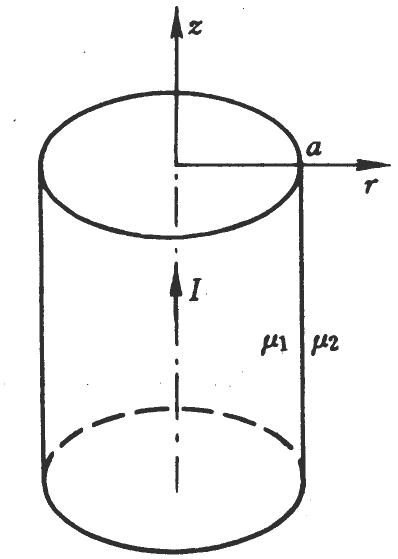
\includegraphics[height=3 cm]{images/q3_1.png}
	\caption{题1.3.3}
\end{figure}
\end{question}

\begin{question}
如图所示,一无限长的磁导率为$\mu_1$的介质圆柱,半径为$R_0$,置于磁导率为$\mu_2$的磁介质中,
在垂直于柱轴方向加一均匀静磁场$\mathbf{H_0}$,求柱内、外磁场分布。

\noindent(在柱坐标系中,$\nabla^2 \phi(r,\theta)=0$的通解为: 
$\phi=c_0 \ln r+d_0+\sum_{n=1}^{\infty}(a_n \cos n\theta+b_n \sin n\theta)(c_nr^n+d_nr^{-n})$,
其中$c_0,d_0,a_n,b_n,c_n,d_n$为常数。)
\begin{figure}[ht]
	\centering
	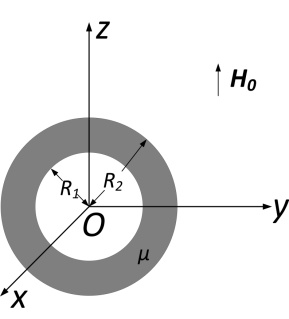
\includegraphics[height=3 cm]{images/q3_2.jpg}
	\caption{题1.3.4}
\end{figure}
\end{question}

\begin{question}
如图所示,有一内、外半径分别为$R_1$和$R_2$的空心球壳,
放置在均匀磁场$\mathbf{H_0}$中,
球壳介质的磁导率为$\mu$,球壳外为真空,求空间的磁标势。
\end{question}


\begin{question}
	一半径为a的均匀带电球壳,质量为M,总电量为Q,
	绕某一直径以角速度$\omega$转动,求磁矩和旋磁比。
\end{question}

\begin{question}
一半径为 a 的均匀带电球壳 ,总电量为 Q ,
绕某一直径以角速度$\omega$转动 ,求磁场总能量 。
\end{question}

\begin{question}
在一长直导线电流$I_1$附近,有一矩形载流线圈,电流为$I_2$,
线圈和直导线的最短距离为x,夹角为$\theta$,
如图所示,计算线圈所受的力和力矩。
\begin{figure}[ht]
	\centering
	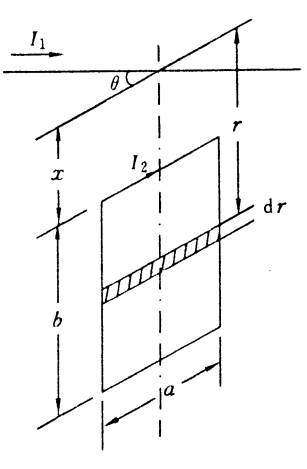
\includegraphics[height=3 cm]{images/q3_3.png}
	\caption{题1.3.8}
\end{figure}
\end{question}